\documentclass[letterpaper,12pt]{article}
\usepackage{tabularx} % extra features for tabular environment
\usepackage{amsmath}  % improve math presentation
\usepackage{float}
\usepackage{graphicx} % takes care of graphic including machinery
\graphicspath{ {./figures/} }
\usepackage[margin=1in,letterpaper]{geometry} % decreases margins
\usepackage{cite} % takes care of citations
\usepackage[final]{hyperref} % adds hyper links inside the generated pdf file
\hypersetup{
	colorlinks=true,       % false: boxed links; true: colored links
	linkcolor=blue,        % color of internal links
	citecolor=blue,        % color of links to bibliography
	filecolor=magenta,     % color of file links
	urlcolor=blue         
}

%++++++++++++++++++++++++++++++++++++++++


\begin{document}

\title{Experiment 3 \protect\\Introduction to Voltage, Current, and Resistance Measurements}
\author{Ahmet Akman 2442366 \protect\\ Assistant : Aybora Köksal}
\date{\today}
\maketitle

%\begin{abstract}
%abstract
%\end{abstract}


\section{Introduction} 
In this experiment, as students, we are expected to experiment with how to use measure voltage, current and resistance by completing the steps described in the third experiment laboratory manual. Throughout these steps, the how to determine the resistance via reading resistor color codes and using multimeter is expected to be learnt. As students, we are expected to discriminate the analog and digital multimeters by taking into account their internal voltage sources. It is observed how to measure the AC line voltage. How to measure DC current and voltage, how the potentiometer works, the characteristics of linear and non-linear resistors ,and equivalent resistances are observed by connecting the multimeters directly to each other and the circuit. The results of the steps were noted and plotted for further comments.

\section{Experimental Results}
In this section, the results of Experiment 3 are discussed.
\subsection{Step 1}
In this step the resistances of the three resistors are read and measured. 
\subsubsection{a} 
The resistances of the resistors are noted after reading them using the color code convention. In Table 1 the values are given. 
\begin{table}[H]
\begin{center}
	\begin{tabular}{||c | c | c||} 
	 \hline
	 Color Order & Value & Tolerance \\ [0.5ex] 
	 \hline\hline
	 Brown / Black / Red / Gold & 1K\( \Omega \) & \( \% \) 5  \\ 
	 \hline
	 Yellow / Violet / Red / Gold & 4.7K\( \Omega \) & \( \% \) 5   \\
	 \hline
	 Brown / Grey / Orange / Gold & 18K\( \Omega \) & \( \% \) 5  \\ [1ex] 
	 \hline
	\end{tabular}
\end{center}
\caption{Resistance reading by color code convention.}
\end{table}

\subsubsection{b} 
The resistances of the resistors are measured using digital multimeter. The measurements are given in the Table 2. 
\begin{table}[H]
	\begin{center}
		\begin{tabular}{||c | c ||} 
		 \hline
		 Resistor & Measured Value \\ [0.5ex] 
		 \hline\hline
		 1K\( \Omega \) & 0.987K\( \Omega \)  \\ 
		 \hline
	     4.7K\( \Omega \) & 4.865K\( \Omega \)   \\
		 \hline
		 18K\( \Omega \) & 17.851K\( \Omega \)  \\ [1ex] 
		 \hline
		\end{tabular}
	\end{center}
	\caption{Resistance reading by color code convention.}
	\end{table}
	

It is observed that the actual value of the resistances can be different than their expected value. This difference could be stemmed from environmental factors as well as probing. Although there are a precision factor the tolerance values are verified. 

\subsection{Step 2}
In Step 2, the digital multimeter instrument  is used only. Using resistance measurement feature of the multimeter, the resistance value of the opposings ends of the 1K and 10K potentiometers are measured. Then The maximum and minimum resistance values between their middle terminals and another terminals are recorded.
The recorded resistance values are provided in the Table 3.
\begin{table}[H]
	\begin{center}
		\begin{tabular}{|| c | c | c | c ||} 
		 \hline
		 Potentiometer & Resistance Between Opposing Ends &  Maximum Resistance & Minimum Resistance\\ [0.5ex] 
		 \hline\hline
		 1K\( \Omega \) & 0.983K\( \Omega \) & 0.981K\( \Omega \) & 0.001\( \Omega \) \\ 
		 \hline
	     10K\( \Omega \) & 8.695K\( \Omega \) & 8.690K\( \Omega \) & 0.004\( \Omega \)  \\
		 \hline
		\end{tabular}
	\end{center}
	\caption{Resistance measurements of the potentiometer}
	\end{table}
It can be inferred that the resistance does not change when we connect the measurement probes to the opposing ends because there is a static resistance between those terminals which approximately corresponds the maximum value of the dynamic terminal.  
\subsection{Step 3}
In this step the internal battery voltages of the analog and digital multimeters are measured and compared.
\subsubsection{a}
Analog multimeter is set for resistance measurement. Then the digital multimeter is set to voltage measurement and its probes are connected to the probes of the analog multimeter. As a result even though the ohmmeter scale is different the measured voltage is observed constant. The measurements are given in the Table 4
\begin{table}[H]
	\begin{center}
		
	
	\begin{tabular}{|| c | c ||}
	\hline
	Scale              & Voltage Value \\[0.5ex] 
	\hline\hline
	x1\( \Omega \)   & -1.5924 V     \\
	\hline
	x10\( \Omega \)  & -1.5924 V     \\
	\hline
	x100 \( \Omega \) & -1.5921 V     \\
	\hline
	x1K\( \Omega \)  & -1.5890 V   \\
	\hline
	\end{tabular}
	\caption{Internal battery measurements of the analog multimeter.}
\end{center}
\end{table}

\subsubsection{b}
Digital multimeter is set for resistance measurement. Then the analog multimeter is set to voltage measurement and its probes are connected to the probes of the digital multimeter. So, the internal battery voltage differs when the digital multimeter set to different ohmmeter scales. The measurements are given in the Table 5.
\begin{table}[H]
	\centering
	\begin{tabular}{|| c | c ||}
		\hline
	Scale & Voltage Value \\\hline
	\hline
	x100 \( \Omega \) & 6V \\\hline
	x1 k\( \Omega \) & 6V \\\hline
	x10 k\( \Omega \) & 6.25 V \\\hline
	x100 k\( \Omega \) & 3V \\\hline
	x1 M\( \Omega \) & 1.5V \\\hline
	x10 M\( \Omega \) & $\sim$0.1 V (or zero) \\\hline
	x100 M\( \Omega \) & $\sim$0.1 V (or zero) \\\hline
	\end{tabular}
	\caption{Internal battery measurements of the digital multimeter.}
\end{table}

This results shows us the digital multimeters are able to adjust its internal voltage when they are measuring resistances in different scales. It can be concluded that digital multimeters have higher precision in measurement.

\subsection{Step 4}
In this step, the line voltage is measured using analog multimeter. Multimeters range is set "500V AC". The measurement is stated in Table 6.
\begin{table}[H]
	\begin{center}
		\begin{tabular}{|| c | c ||} 
		 \hline
		 Line Voltage & Approximately 220\(V_{ac}\) 		 \\ [0.5ex] 
		
		 \hline
		\end{tabular}
	\end{center}
	\caption{Line voltage measurement }
\end{table}

\subsection{Step 5}
In Step 5, power supply and digital multimeter instruments are used. The circuit in the Figure 1 is constructed on the breadboard. 
\begin{figure}[H]
	\caption{Circuit schematic for the step 5}
	\centering
	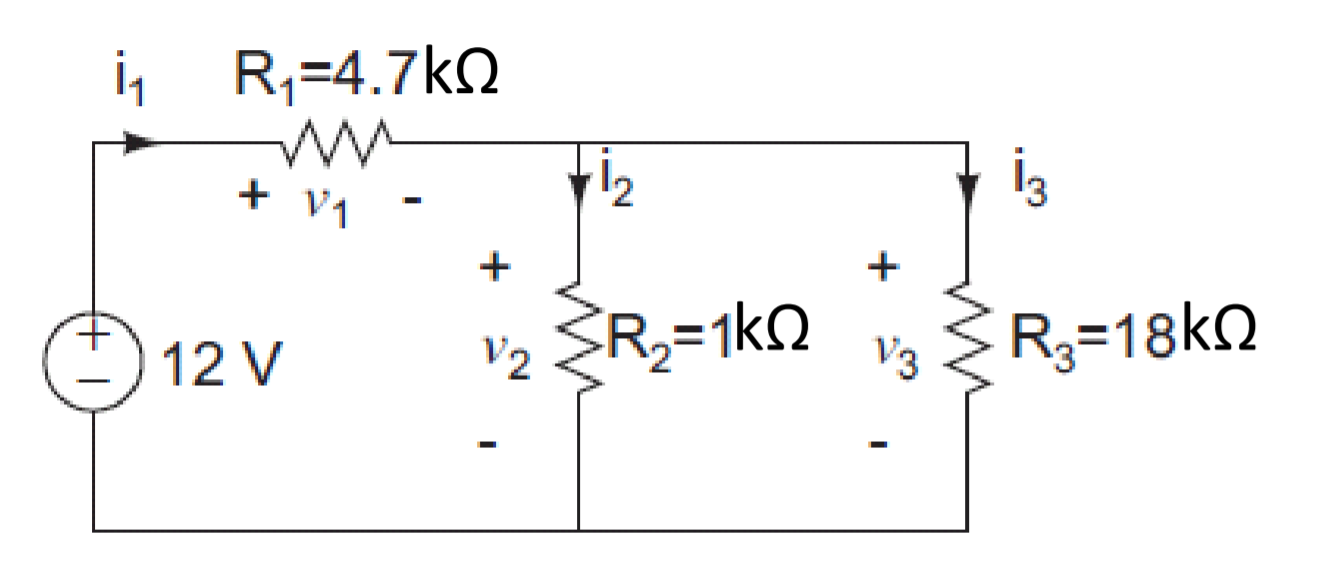
\includegraphics[width=0.6\textwidth]{5.png}
\end{figure} 
Then the required voltage and current measurements are made. The measurements are given in the Table 7.
\begin{table}[H]
	\centering
	\begin{tabular}{|| c | c | c ||}
		\hline
	\(V_1\) & \(V_2\) & \(V_3\) \\
	\hline
	10.041V & 1.948V & 1.948 \\
	\hline\hline
	\(i_1\) & \(i_2\) & \(i_3\) \\
	\hline
	2.064mA & 1.957mA & 0.109mA\\
	\hline
	\end{tabular}
	\caption{Voltage and current measurements for the step 5}
	
	\end{table}

\subsection{Step 6}
In this step, power supply , analog multimeter ,and digital multimeter instruments are used. The circuit illustrated in Figure 2 is set. 

\begin{figure}[H]
	\caption{Circuit schematic for the step 6}
	\centering
	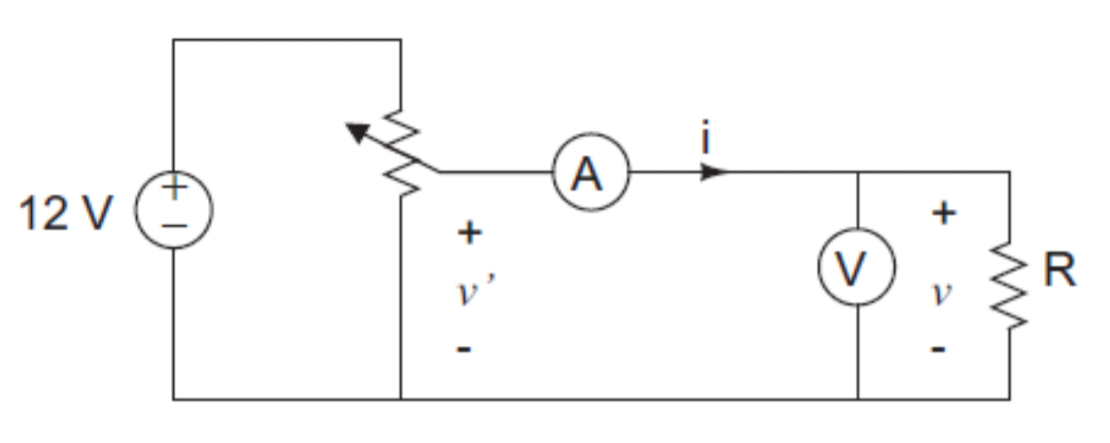
\includegraphics[width=0.6\textwidth]{6.png}
\end{figure} 

The resistor with resistance "R" is selected as "4.7K\(\Omega\)". The potentiometer is adjusted so that the voltage value becomes 9, 7, 5, 0 volts. For all cases the current \emph{i} is measured and recorded.

\subsubsection{a}
The current and voltage measurements are made and plotted in MATLAB. The Figure 3 shows  \emph{i} versus \emph{v}. The resistor with resistance "R" is measured as approximately "4.602k\(\Omega\)" using the equation " R  = \(\frac{V}{I}\) ".

\begin{figure}[H]
	\caption{Plot of \emph{i} versus \emph{v}}
	\centering
	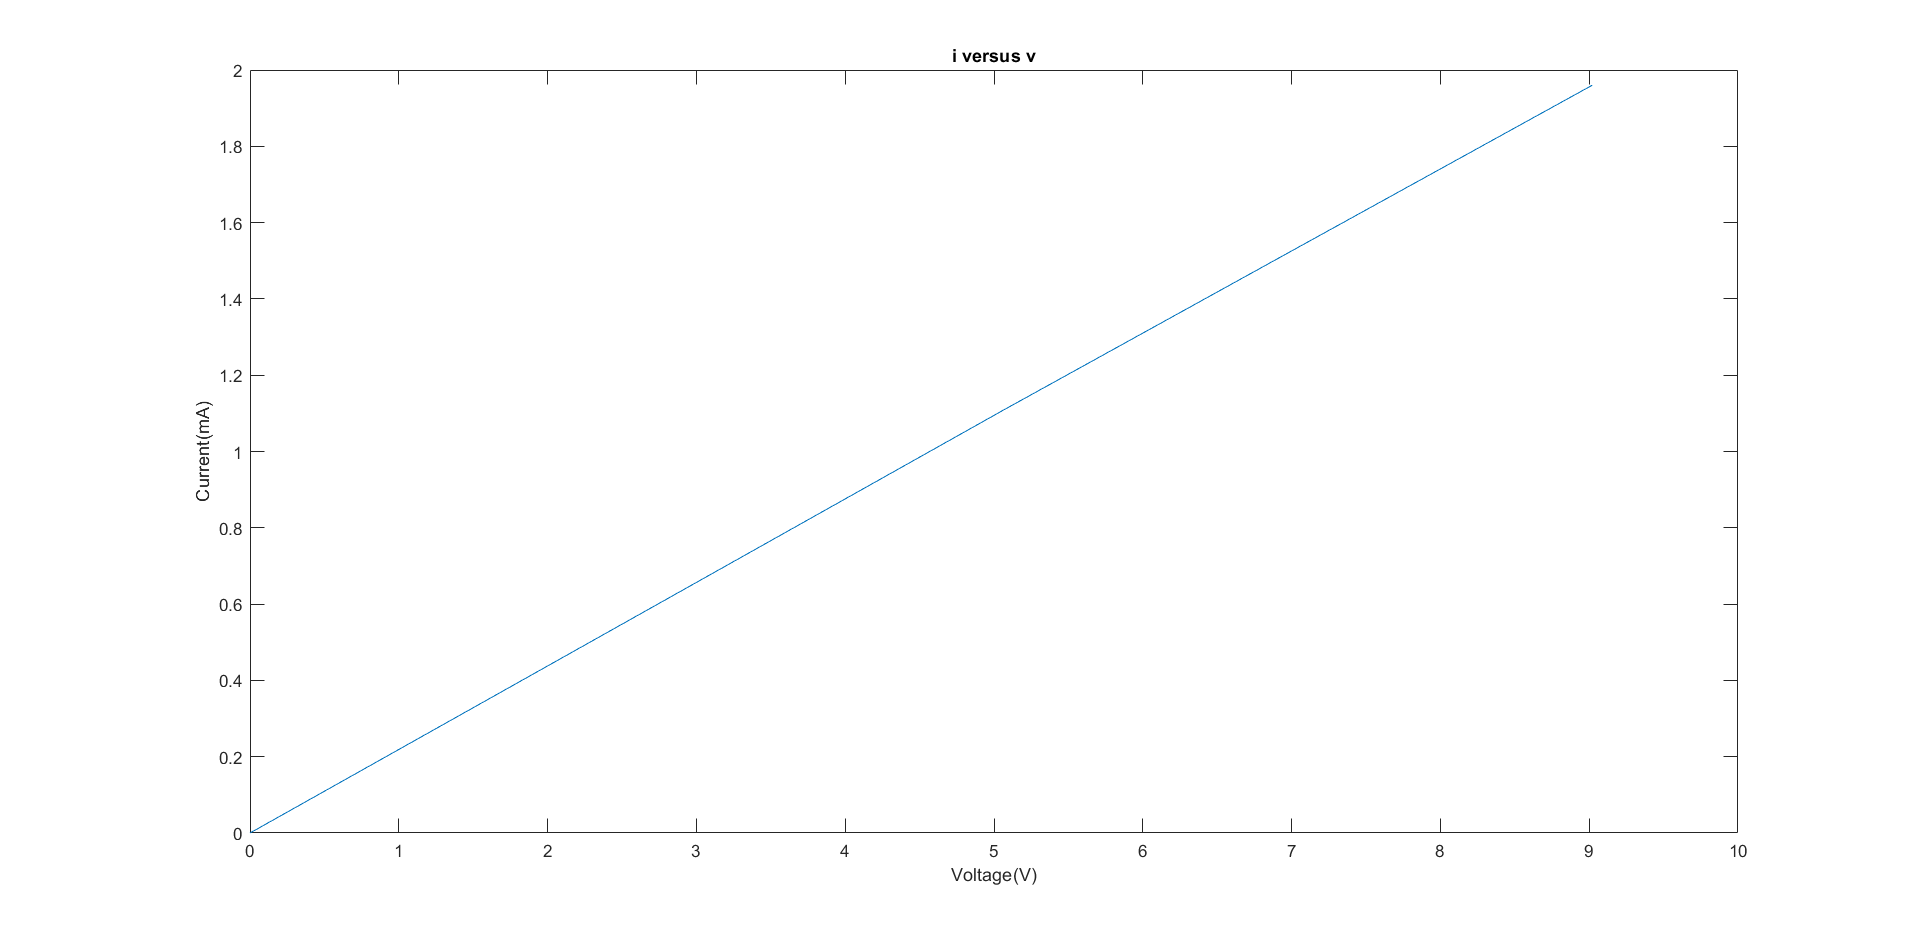
\includegraphics[width=1\textwidth]{6a.png}
\end{figure} 


\subsubsection{b}

The resistor with resistance "R" is measured as approximately "4k\(\Omega\)" using analog multimeter.
\subsubsection{c}

The resistor with resistance "R" is measured as  "4.60k\(\Omega\)" using digital multimeter.

\subsubsection{d}
It can be seen from the Figure 3 that the plot is approximately linear. This is because the equation of  \emph{ R (constant) = \(\frac{V}{I}\) } . Also the measurements from the analog and digital multimeters practically shows that the digital multimeters have higher resolution ,whose measurement is approximately same with the experimental and given resistance data.

\subsection{Step 7}



\section{Conclusion}
In conclusion, in experiment 2, "Signal Generators and Oscilloscopes," as students, we have learned how to use the signal generator and oscilloscopes instruments' behavior under nine steps. The scaling and movement properties of the oscilloscope channels are explored on a square waveform then the difference between "AC" and "DC" coupling methods are observed and explained. Also, inversion of the signal is observed then interpreted. The experiment repeated for the second channel, and the results are verified. Using cursor functions of the DSO, various measurements are made. The measurement features of the oscilloscope instrument are experienced. Different circuits are set and supplied by the signal generator, and the outputs are observed and plotted using DSO. The outputs of the function waveform generator and the prob comparison port of the oscilloscope are compared, and the trigger signal effect of the DSO is observed so that both signals are fit to the same time frame steady. Lastly, the mathematical operation ability is used to add and subtract the signals, then the results are observed.  In this experiment, as students, we have experimented with how to use signal generators and oscilloscopes.


assdasd \( \Omega \) A


\section*{Appendix I}
Total time spent on/during:
\begin{itemize}
	\item Pre-lab preparation: 1 hours (including the preliminary work and simulations) 
	\item Experimental work: 2 hours (hours spent in lab)
	\item Report writing: 8 hours 
\end{itemize}
%++++++++++++++++++++++++++++++++++++++++
% References section will be created automatically 
% with inclusion of "thebibliography" environment
% as it shown below. See text starting with line
% \begin{thebibliography}{99}
% Note: with this approach it is YOUR responsibility to put them in order
% of appearance.

%\begin{thebibliography}{99}

%https://tr.overleaf.com/latex/templates/sample-lab-report-for-u-of-r-phys-349/pgsyqngcyjxk

%\end{thebibliography}


\end{document}